% !TEX root = MAIN.tex

\section{Mutation Testing Process}
\label{sec:process}

	\begin{figure}
	\centering
		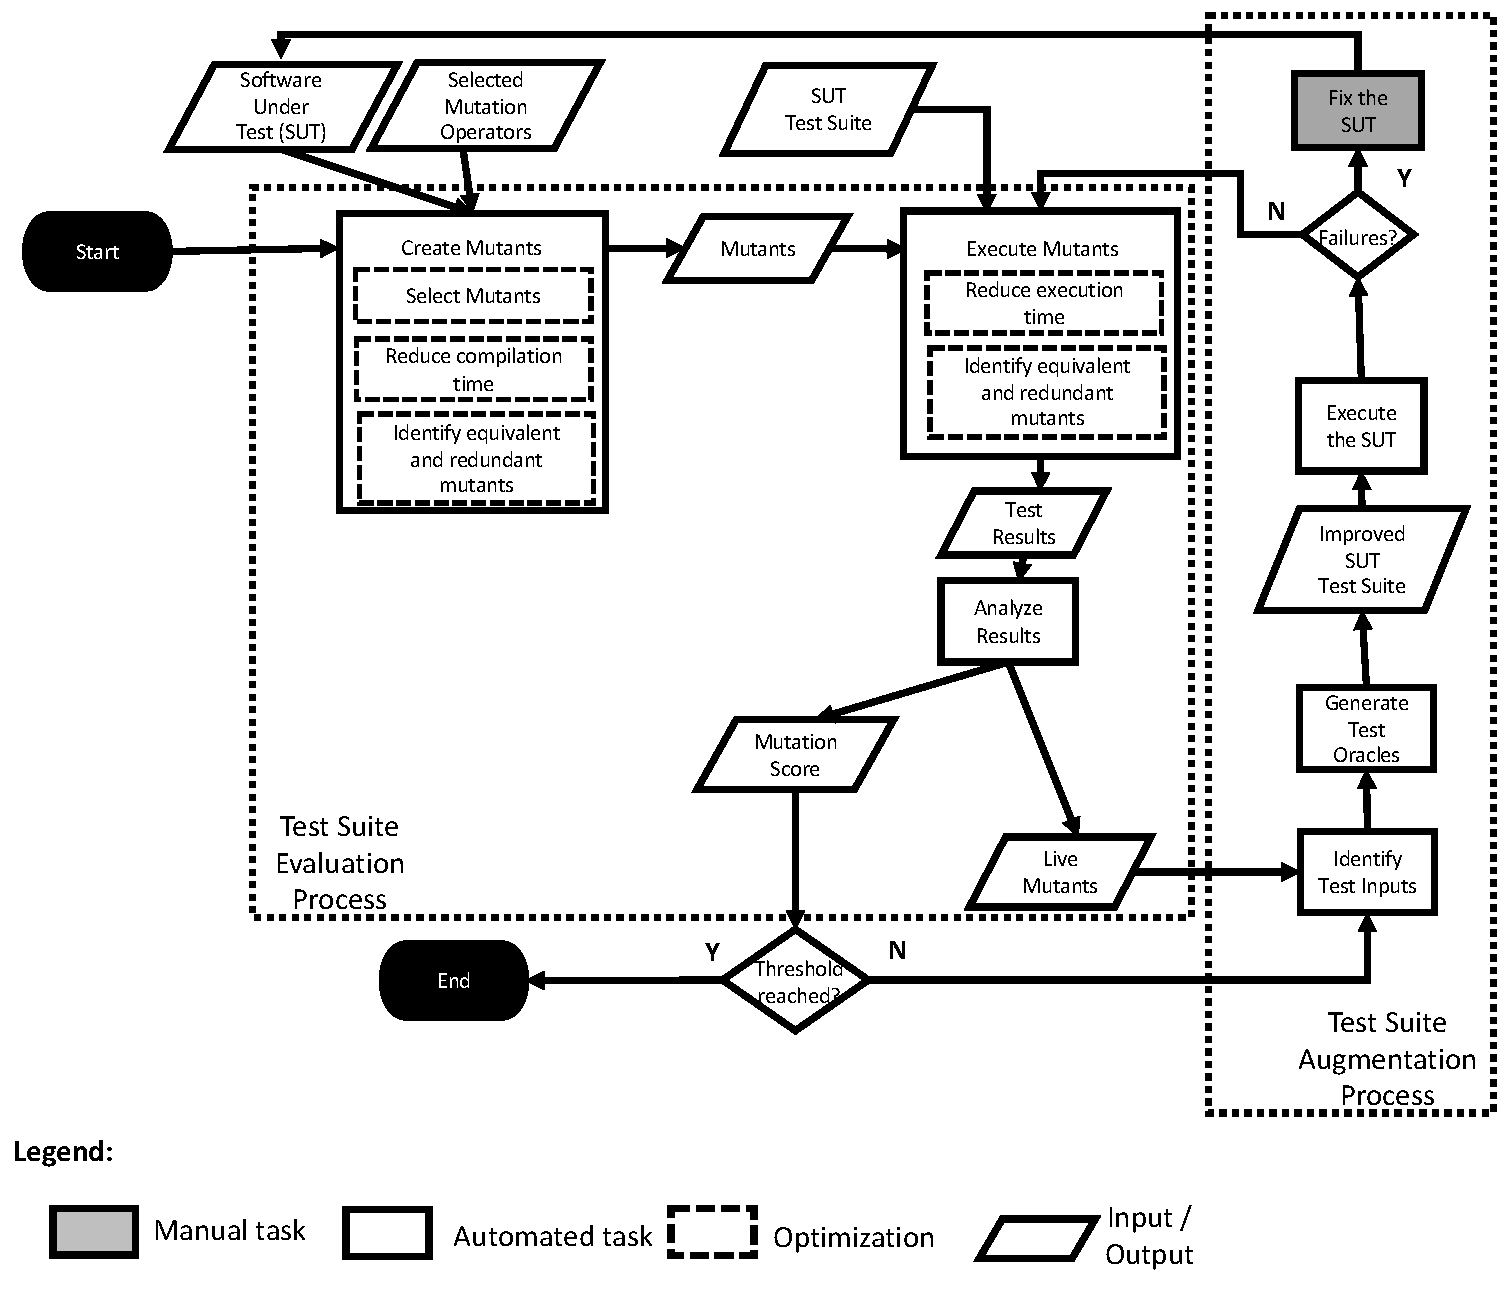
\includegraphics[width=\textwidth]{images/process}
		\caption{Mutation Testing Process.}
		\label{fig:code:process}
	\end{figure}

Figure~\ref{fig:code:process} shows the reference \INDEX{code-driven mutation testing process} that will be considered in this book. The process depicted in Figure~\ref{fig:code:process} has been inspired by the mutation testing process described in related work~\cite{offutt2001mutation,papadakis2019mutation}, it has been presented in deliverable D1. The process is based on two main sub-processes, \emph{test suite evaluation} and \emph{test suite augmentation}, which are described in Sections~\ref{sec:testSuiteEvaluation:codeDriven}~and~\ref{sec:testGeneration:codeDriven}, respectively.


\endinput




